
\documentclass[tikz, border=10mm]{standalone}
\usepackage{xcolor}
\usepackage{tikz}
\usetikzlibrary{positioning, calc, backgrounds, quotes, arrows.meta}

% Color Definitions (Matching nn_blocks.tex)
\definecolor{ConvColor}{rgb}{0.98,0.81,0.69}
\definecolor{PoolColor}{rgb}{0.8,0.33,0.33}
\definecolor{UnpoolColor}{rgb}{0.6,0.7,0.9}
\definecolor{FcColor}{rgb}{0.6,0.2,0.8}
\definecolor{ResBlockColor}{rgb}{0.85,0.92,1.0}

% 3D Style Approximation
\tikzset{
    box3d/.style={
        shape=rectangle,
        draw=black!50,
        fill=#1,
        minimum width=1cm,
        minimum height=1.5cm,
        append after command={
            \pgfextra{
                \draw[fill=#1!80!black, draw=black!50] (\tikzlastnode.north east) -- ++(0.3,0.3) -- ++(-1,0) -- (\tikzlastnode.north west) -- cycle;
                \draw[fill=#1!60!black, draw=black!50] (\tikzlastnode.north east) -- ++(0.3,0.3) -- ++(0,-1.5) -- (\tikzlastnode.south east) -- cycle;
            }
        }
    }
}

\begin{document}
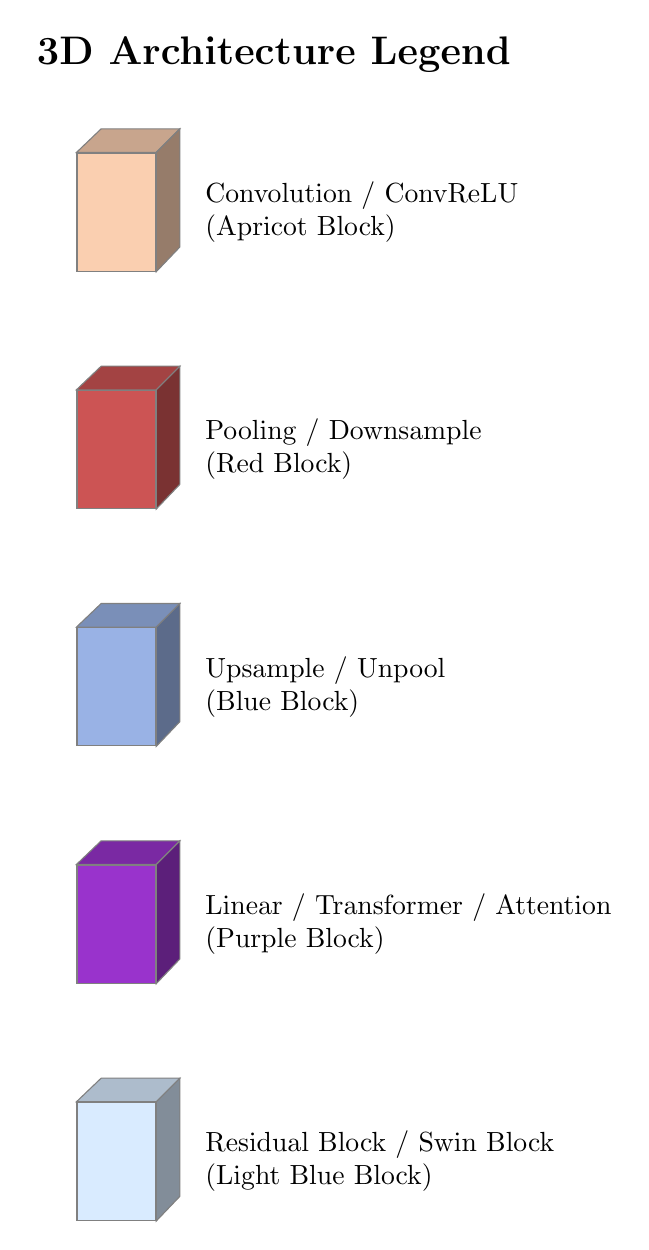
\begin{tikzpicture}[node distance=0.8cm, every node/.style={transform shape}]

% Title
\node[font=\Large\bfseries] at (2, 7) {3D Architecture Legend};

\coordinate (start) at (0, 5);

% Conv
\node[box3d=ConvColor] (l_conv) at (start) {};
\node[right=0.5cm of l_conv, align=left] {Convolution / ConvReLU\\(Apricot Block)};

% Pool
\node[box3d=PoolColor, below=1.5cm of l_conv] (l_pool) {};
\node[right=0.5cm of l_pool, align=left] {Pooling / Downsample\\(Red Block)};

% Up
\node[box3d=UnpoolColor, below=1.5cm of l_pool] (l_up) {};
\node[right=0.5cm of l_up, align=left] {Upsample / Unpool\\(Blue Block)};

% FC
\node[box3d=FcColor, below=1.5cm of l_up] (l_fc) {};
\node[right=0.5cm of l_fc, align=left] {Linear / Transformer / Attention\\(Purple Block)};

% Res
\node[box3d=ResBlockColor, below=1.5cm of l_fc] (l_res) {};
\node[right=0.5cm of l_res, align=left] {Residual Block / Swin Block\\(Light Blue Block)};

\end{tikzpicture}
\end{document}
